%% Chapter Trigger

\chapter{Sistema de Filtragem do ATLAS}

O ATLAS apresenta três níveis de seleção de eventos: Primeiro Nível~(L1),
Segundo Nível~(L2) e o \emph{Event Filter}~(EF). O L2 e o EF juntos são chamados
de \emph{High Level Trigger} (HLT). O L1 é implantado utilizando placas
eletrônicas especialmente projetadas para a tarefa, enquanto o HLT é quase 
totalmente composto por dispositivos de rede e computadores disponíveis
comercialmente~\cite{ref:2010performance}.

O L1 procura por assinaturas de múons com momento elevado, elétrons/prótons e
jatos. Nesta fase, são considerados apenas detectores com granularidade restrita
como, o RPC do múon e os subsistemas dos calorímetros eletromagnético e
hadrônico~\cite{LEVEL1TRIGGER}. A taxa máxima de aquisição projetada para o L1 é
igual a 75~kHz, e pode ser aumentada até 100~kHz após uma atualização do
sistema~\cite{ATLAS2008}. A decisão de rejeitar ou não um evento deve ser tomada
dentro de 2,5~$\mu$s após a tomada de dados.

O L2 é alimentado pelas RoIs. Essas são as regiões do detector ATLAS onde o L1
identificou possíveis objetos de interesse. O L2 usa as coordenadas, a energia e
o tipo de assinatura para limitar a quantidade de dados que será transmitida
dos instrumentos de leitura do detector. Nesse momento, a taxa de eventos cai
para 3,5~kHz, com um processamento médio de aproximadamente
40~ms~\cite{ATLAS2008}.

O EF usa análise \emph{offline} de eventos já reconstruídos para reduzir a taxa
de armazenagem para cerca de 200~Hz. Os eventos selecionados e gravados serão
utilizados em análises subsequentes~\cite{ARMSTRONG2004}. A
Figura~\ref{fig:triggersystem} representa graficamente o fluxo de informações do
sistema de filtragem.

\begin{figure}[htpb!]
    \centering
    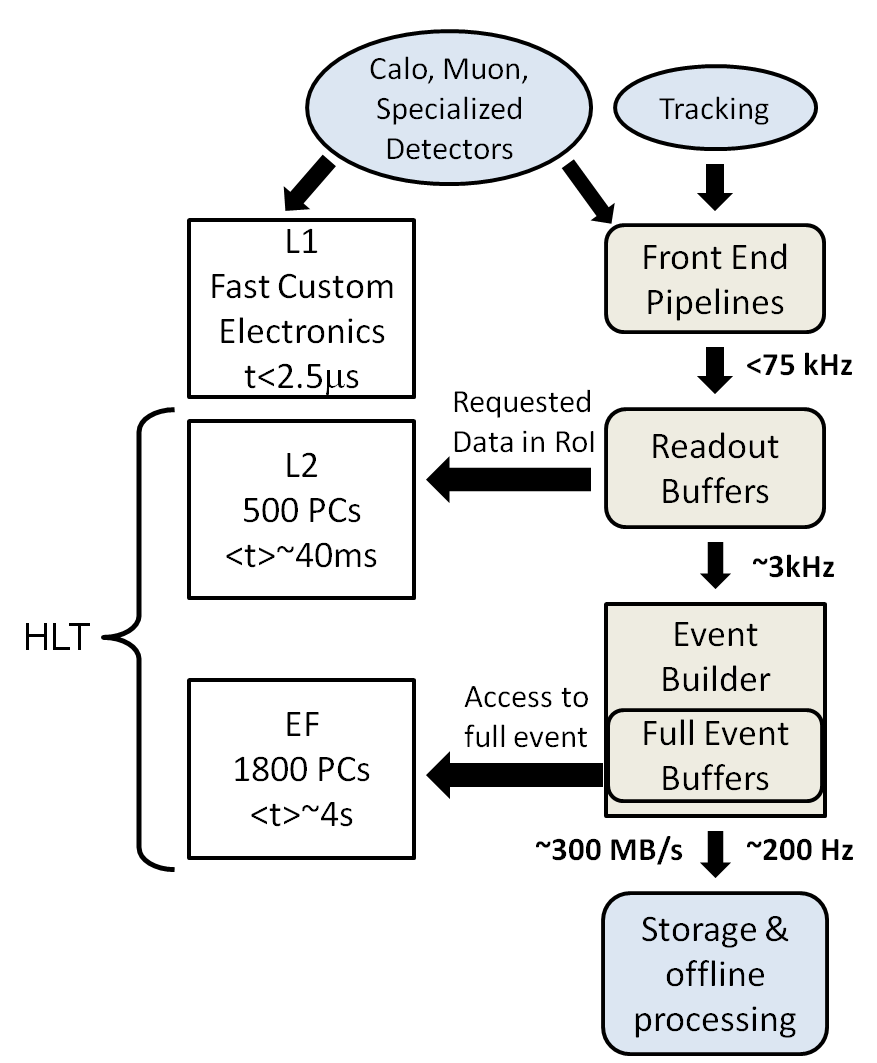
\includegraphics[width=8cm]{images/atlas_trigger_system.png}
    \caption[Esquemático do sistema de filtragem do ATLAS.]{Esquemático do
    sistema de filtragem do ATLAS. Extraído de~\cite{ref:2010performance}.}
    \label{fig:triggersystem}
\end{figure}

Os algoritmos utilizados no HLT usam a granularidade e precisão máxima para os
dados dos calorímetros e câmaras de múon, além de dados provenientes do
detector de traços para refinar a seleção~\cite{ATLAS2008}. Quanto mais
informações sobre a energia depositada, melhor a determinação de limiares de
corte. Já a reconstrução da trajetória na parte mais interna do detector
permite a diferenciação de partículas, como, por exemplo, elétrons e prótons.

O sistema de aquisição de dados (DAQ, do inglês \emph{Data AcQuisition} ) recebe
os eventos, na mesma taxa do que no L1, e retêm-os em um \emph{buffer}.
Posteriormente, os dados são transmitidos através de uma comunicação
ponto-a-ponto~\cite{ATLAS2008}.  Qualquer informação requerida pelo L2 é
transmitida, geralmente relacionadas às RoIs. Os eventos que passarem por todos
os critérios de seleção do L2 serão compilados (o chamado \emph{event-building})
e passados pelo DAQ para o EF~\cite{ATLAS2008}. Finalmente, os eventos
selecionados serão armazenados permanentemente~\cite{VAN2009}.

Para controlar todo tráfego de dados durante a cadeia de seleção, o DAQ ainda
fornece a configuração, controle e monitoramento do detector ATLAS durante a
tomada de dados~\cite{ATLAS2008,MIOTTO2010}.

O sistema de controle do detector (DCS,  do inglês \emph{Detector Control
System}) é o responsável pela supervisão e operação do \emph{hardware} (sistema
de gás, fontes de alimentação, sistema de refrigeração, etc.)~\cite{PPOY2008}.

\section{Primeiro Nível de Filtragem}

O fluxo de dados do L1 é mostrado na Figura~\ref{fig:l1schema}. Nesse nível, a
seleção inicial é realizada baseada na informação dos calorímetros e do
espectrômetro de múon.

\begin{figure}[htpb!]
    \centering
    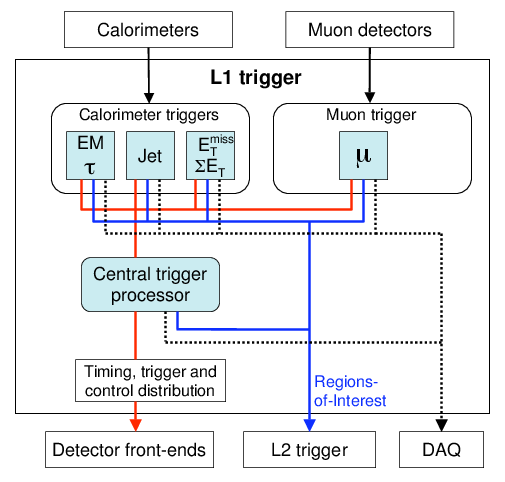
\includegraphics[width=8cm]{images/l1-schema.png}
    \caption[Diagrama de blocos do L1.]{Diagrama de blocos do L1. As decisões do L1 são tomadas no
    CTP~(Processador de Filtragem Central), tomando em conta os resultados dos
    sistemas de calorimetria e de múons. O fluxo para a eletrônica de
    \emph{front-end}, para o L2 e para o DAQ, são mostradas em vermelho, azul e
    preto, respectivamente. Retirado de ~\cite{ATLAS2008}.}
    \label{fig:l1schema}
\end{figure}

O L1 de calorimetria (L1Calo) tem como principal objetivo na identificação de
partículas como elétrons, fótons, jatos e o $\tau$-léptons\footnote{O
$\tau$-lépton, ou simplesmente tau, é uma partícula elementar similar ao
elétron, com carga elétrica negativa e spin de
$\frac{1}{2}$~\cite{ATLAS2011TAU}.} que decaiam em hádrons. Eventos com grande
energia transversa também são almejados. 

O L1 do sistema de múon baseia-se nos sinais das câmaras de trigger: RPCs na
região do barril e TGC's no \emph{end-caps}. A seleção ocorre através de
padrões consistentes com múons com alto momento transverso originados na região
de interação. Sua lógica disponibiliza 6 limiares para $p_T$
independentes~\cite{ATLAS2008}. A informação que o L1 disponibiliza é a
quantidade de múons que atingiram cada limiar. É importante ressaltar que nunca
um múon é contado em dois limiares diferentes~\cite{ATLAS2008}.


As decisões tomadas pelo L1 são feitas no Processador de  Filtragem
Central~(CTP, do inglês \emph{Central Trigger Processor}), que combina as
informações de todos os tipos de objetos.  Dependendo das características
extraídas, o evento é classificado em até 256 itens separados. A
Tabela~\ref{table:l1objects} apresenta um resumo dos objetos disponíveis para
L1, os limiares de seleção e suas respectivas frequências obtidas em 2012.

\begin{table}[htbp!]\footnotesize
  \centering
  \tabcolsep=0.08cm
  \begin{tabular}{ l  m{5cm} c c }
      \toprule
                                          & Objeto de interesse & Limiar de seleção (GeV) & Frequência~(kHz) \\
      \midrule
      \multirow{2}{*}{Léptons simples}    & Múon $p_T > 25$~GeV        &      15             & 8        \\
                                          & Elétron $p_T > 25$~GeV     &      18             & 17       \\
      \midrule
      \multirow{4}{*}{Léptons duplos}     & 2 Múons $p_T > 15$~GeV     &      2x10           & 1        \\
                                          & 2 Múons $p_T > 20,10$~GeV  &      15             & 8        \\
                                          & 2 Elétrons $p_T > 15$~GeV  &      2x10           & 6        \\
                                          & 2 Taus $p_T > 45$~GeV      &      15, 11         & 12       \\
      \midrule
      \multirow{2}{*}{Fótons  duplos}     & 2 Fótons $p_T > 25$~GeV    &   2x10              & 6        \\
                                          & 2 Fótons \emph{loose} $p_T > 40,30$~GeV & 12, 16 & 6        \\
      \midrule
      Outros                              &                            &                     & $\sim 6$ \\
      \midrule
      {\bf Total}                         &                            &                     & $\sim 75$ \\
      \bottomrule
  \end{tabular}
  \caption[Taxa de eventos para os objetos de interesse no L1.]{Taxa de eventos
  para os objetos de interesse no L1. Retirado de~\cite{PETERSEN}.}
  \label{table:l1objects}
\end{table}

Neste ponto, apenas o número de ocorrências de objetos selecionados é levado em
consideração (ou \emph{flags} indicando quais limiares foram alcançados). As
informações sobre a localização geométrica de um objeto é retida nos
processadores de \emph{trigger} dos sistemas de calorimetria e de múons. Assim
que o evento for aceito no L1, essas informações serão mandadas como RoIs para o
L2, onde serão usadas no processo de seleção.

Uma função fundamental do L1 é identificar o \emph{bunch-crossing} de interesse.
O \emph{bunch-crossing}, ou simplesmente BC, é o termo atribuído à injeção de
pacotes de prótons no acelerador ocorrida a cada 25~ns. Este curto espaço de
tempo torna a tarefa um desafio. No caso do \emph{trigger} do múon, o tamanho do
detector implica em um tempo de percurso maior que o intervalo entre as injeções
de pacote. Já os sinais de calorimetria duram tipicamente quatro vezes mais que
o \emph{bunch-crossing}~\cite{ATLAS2008}.

Enquanto a decisão do \emph{trigger} é realizada, as informações de todos os
canais do ATLAS estão armazenadas em memória. Essas memórias estão localizadas
na eletrônica de \emph{front-end} e frequentemente está submetida a altos
níveis de radiação, onde o acesso é muito difícil~\cite{ATLAS2008}. É desejável
que o \emph{pipeline} de memória seja o menor possível. O projeto da eletrônica
de \emph{front-end} requer que essa latência seja de no máximo 2,5~$\mu$s.
Cerca de 1~$\mu$s desse tempo é deixado para propagação dos dados no
cabeamento.

\subsection*{Primeiro Nível de Filtragem da Calorimetria}

As 7.000 saídas analógicas dos calorímetros eletromagnético e hadrônico são
tratadas pelo \emph{L1Calo}. A Figura~\ref{fig:L1CALO} apresenta sua
arquitetura. Este é um sistema digital localizado na parte externa do ATLAS
constituído por 3 subsistemas:

\begin{figure}[htpb!]
    \centering
    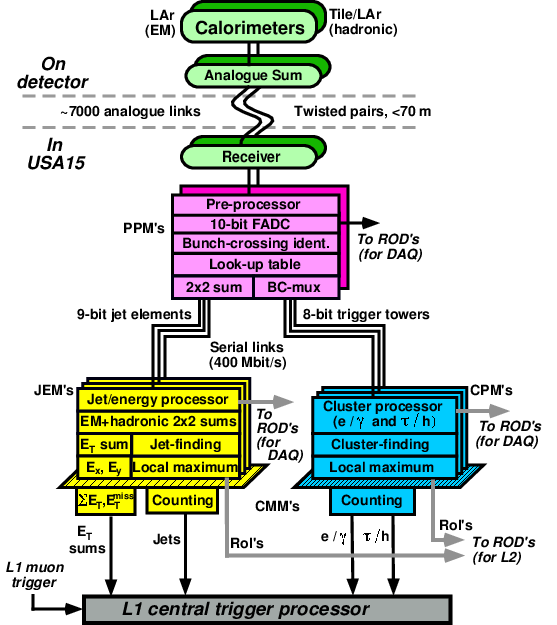
\includegraphics[width=12cm]{images/CaloTrigArch.png}
    \caption[Esquemático do funcionamento do \emph{L1Calo}.]{Esquemático da
    arquitetura do \emph{L1Calo}~(Extraído de~\cite{ATLAS2008}).}
    \label{fig:L1CALO}
\end{figure}


\begin{description}
    \item[Módulo de pré-processamento] Responsável por digitalizar os sinais
    analógicos recebidos e utiliza um filtro que os associa com o
    \emph{bunch-crossing} específico. Utiliza  ainda uma tabela de
    referência para fornecer os valores de energia transversa que serão usados
    nos algoritmos subsequentes.
    \item[Processadores de \emph{clusters}~(CP)] Responsável por identificar
    candidatos a elétrons/prótons e $\tau$-léptons através de limiares
    relacionados a deposição de energia.
    \item[Processadores de Jatos e Energia~(JEM)] Recebe elementos de interesse
    e os usa para identificar jatos e calcular a energia transversa total.
\end{description}

 A descrição completa de cada um dos blocos e da eletrônica responsável por essa
 etapa da filtragem de eventos pode ser encontrada em~\cite{ACHENBACH2008}.



\section{Sistema de Filtragem de Alto Nível}

O sistema de filtragem de alto nível do ATLAS (\emph{High Level Trigger} - HLT)
é composto pelo L2  e EF, ambos implementados em \emph{software} com linguagem
de programação de alto nível. A Figura~\ref{fig:tdaq_diagram} apresenta os
detalhes desta parte do sistema de filtragem. O HLT
está dividido em duas partes: a aquisição e controle de dados e o
processamento dos eventos produzidos pelo ATLAS. Estas duas partes, juntas, são
referidas como TDAQ (\emph{Trigger and Data Aquisition})~\cite{NEGRI2012,ref:TORRES}.

\begin{figure}[hbtp!]
\centering
    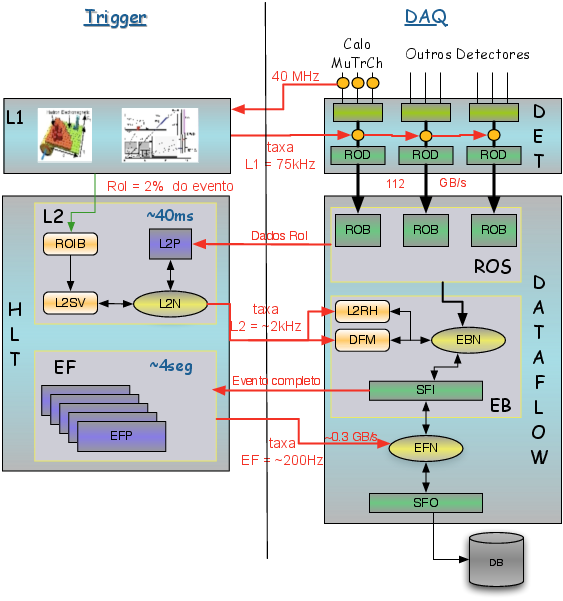
\includegraphics[height = 10cm]{images/tdaq_diagram.png}
    \caption[Diagrama em blocos do sistema de filtragem de alto nível.]{Diagrama
    em blocos do sistema de filtragem de alto nível (Retirado
    de~\cite{TORRES2009}).}
    \label{fig:tdaq_diagram}
\end{figure}


Após a filtragem do L1, os eventos aprovados ficam disponíveis na forma de
fragmentos nos sistemas de leitura (\emph{Read-Out Systems - ROS}).  Além
disso, a informação a respeito das RoIs etiquetadas pelo L1 é enviada para o
construtor de RoI (\emph{RoI Builder} - RoIB). Este agrupa os fragmentos de
informação gerados pelos diferentes detectores do ATLAS e transmite o registro
gerado por este agrupamento para um supervisor do segundo nível (\emph{L2
Supervisor - L2SV}), que ficará responsável por atribuir a RoI recebida a uma
unidade de processamento do segundo nível  (\emph{L2 Processing Unit} - L2PU).
A L2PU então valida a etiqueta do L1, usando a plena granularidade dos
detectores, e retorna o resultado para o L2SV. Este envia o resultado para o
gerenciador de fluxo de dados (\emph{Dataflow Manager - DFM}), para que o
evento seja apagado em caso de rejeição, ou propagado para o filtro de eventos,
caso seja aprovado.  O DFM seleciona um dos processadores SFI (\emph{Sub-Farm
Input}) para que o mesmo solicite aos ROS toda a informação disponível do
evento em questão. Uma vez a informação disponível, o SFI seleciona um dos
processadores do filtro de eventos (\emph{EF Processor - EFP}), para que o
mesmo realize análises detalhadas, usando toda a informação disponível para
cada evento, gerando, assim, a decisão final do sistema de filtragem. Os
eventos finalmente aprovados são enviados aos processadores SFO (\emph{Sub-Farm
Output}) para que possam ser armazenados em mídia permanente, permitindo
posterior análise \emph{offline}~\cite{RIU2008}.

Todo o segundo nível de filtragem foi desenvolvido utilizando, o máximo
possível, tecnologias padronizadas (comerciais)~\cite{ANJOS2004}, visando
fácil reposição de material e implementação simplificada. Todos os
processadores são de uso geral (tipo PC) e praticamente todas as comunicações
entre estes dispositivos são feitas através de \emph{switchs} Gigabit Ethernet,
devido à velocidade, confiabilidade e padronização do protocolo. Todas as
aplicações também estão desenvolvidas utilizando técnicas de orientação a
objetos e implementadas em C++~\cite{SCHILDT2003}.


\section{Seleção de Múons}

Múons detectados pelo RPC, no L1, alimentam os algoritmos do HLT (High-Level
Trigger). Além de utilizar informação com granularidade fina, estes algoritmos
tem acesso à informação de trajetória do ID (\emph{Inner Detector}) e da energia
perdida pelo múon nos calorímetros. Com isso, não só o momento transverso do
múon pode ser refinado, mas também informações sobre a origem física desse múon.
Essas informações são necessárias para a identificação dos processos físicos que
aconteceram no detector.

\subsection{Seleção no L1}

O primeiro nível de filtragem para múons, conhecido como \emph{L1Muon}, busca
pela combinação de cruzamentos entre partículas e as diferentes câmaras do
espectrômetro, afim de identificar múons em 6 patamares de momento
transverso~($p_T$) distintos.

Ao detectar o cruzamento de um múon na primeira estação, o sistema projeta
janelas de visualização nas outras camadas. Estas janelas foram pré-calculadas
usando simulações de Monte Carlo. Cada combinação de pontos de cruzamento indica
o $p_T$ da partícula~\cite{BUTTINGER2012}. Aproximadamente 15~kHz dos 75~kHz da
banda de seleção do nível 1 de filtragem são reservados para eventos de múons. A
Figura~\ref{fig:MSMUON} mostra dois exemplos de múons passando pelo
espectrômetro. Nela está representada uma seção transversal do detector ATLAS e
a representação de duas janelas de visualização projetadas pelo sistema de
filtragem: uma para um múon de baixo $p_T$ e outra para o de alto $p_T$.


\begin{figure}[htpb!]
    \centering
    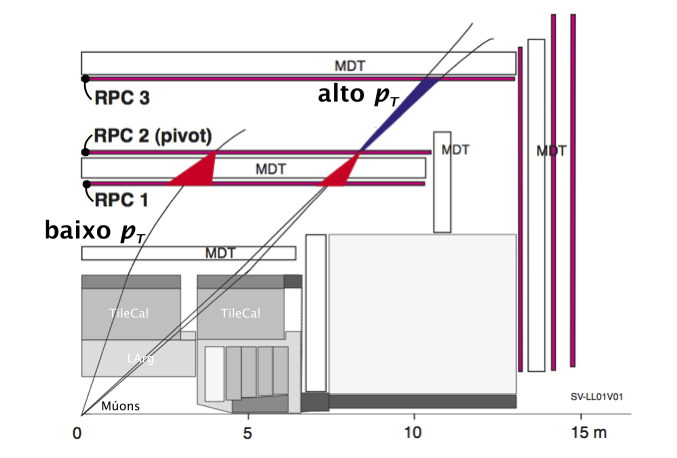
\includegraphics[width=11cm]{images/MS_transversal.png}
    \caption[Seção transversal do detector ATLAS, mostrando exemplos de duas
    partículas cruzando as câmaras do espectrômetro e as respectivas projeções
    do \emph{L1Muon}]{Seção transversal do detector ATLAS, mostrando exemplos de duas
    partículas cruzando as câmaras do espectrômetro e as respectivas projeções
    do \emph{L1Muon} (Adaptado de~\cite{BUTTINGER2012}).}
    \label{fig:MSMUON}
\end{figure}

O \emph{L1MUON} é configurado para encontrar os seguintes patamares de
seleção~\cite{BUTTINGER2012}:

\begin{description}
    \item[MU0] Aceita múons com qualquer valor de $p_T$. Basta a partícula
    cruzar duas estações do mesmo setor do espectrômetro. Esse patamar foi
    substituído pelo MU4 a partir da metade de 2011.
    \item[MU4] Seleciona múons que cruzam duas estações de coincidência do mesmo
    setor com $p_T$ aproximadamente igual a 4~GeV.
    \item[MU6] Seleciona múons com $p_T$ acima de aproximadamente 6~GeV. Requer
    que pelo menos duas estações do RPC sejam atingidas ou as três coincidências
    no TGC.
    \item[MU10] Seleciona múons com $p_T$ acima de aproximadamente 10~GeV. Possui
    as mesmas regras de coincidência do MU6, porém projeta janelas menores.
    \item[MU11] Seleciona múons com $p_T$ acima de aproximadamente 11~GeV. Exige
    três coincidências em todas as regiões (RPC ou TGC) do sistema. Não existe
    resolução suficiente de energia para diferenciar os patamares MU11 e MU10.
    \item[MU15] Seleciona múons com $p_T$ acima de aproximadamente 15~GeV. Exige
    a passagem do múon nas três estações.
    \item[MU20] Seleciona múons com $p_T$ acima de aproximadamente 20~GeV. Possui
    as mesmas regras de coincidência do MU15, porém projeta janelas menores.
\end{description}

Algumas regiões do detector não são cobertas pelo RPC devido a questões
geométricas~\cite{MUONTDR1997}. Nessas regiões, o múon não pode ser classificado
como MU11, MU15 ou MU20, mesmo que o valor de $p_T$ o qualifique para tal
patamar. Adicionalmente, cerca de 1\% das placas RPC pararam de funcionar devido
à problemas no sistema de alimentação~\cite{ATLAS-CONF-2012-099}, aumentando
assim o número de regiões sem cobertura. Nesses casos, os eventos são marcados
como MU10.

A partir de 2011, observou-se um aumento na taxa de múons marcados com MU10.
Isso deve-se a instalação de uma blindagem adicional entre a região dos barris e
os \emph{end-caps}.

\subsection{Seleção no HLT}

A seleção de múons no L2 utiliza informações com granularidade plena para as
RoIs passadas pelo L1, melhorando a estimativa da posição e do momento
transverso atráves de algoritmos otimizados para uma rápida seleção e uma
eficiente rejeição de ruído de fundo~\cite{VENTURA2010}. Ao invés de utilizar a
informação proveniente do RPC, esses algoritmos processam dados adquiridos
pelas câmaras de precisão (MDT no caso da região do barril). Os algoritmos do EF
também tem acesso à resolução pena do detector~\cite{KORDAS2007}.


A Figura~\ref{fig:MUONHLTFLOW} apresenta o fluxo de dados entre os diversos algoritmos de
seleção de múons do L1, L2 e EF. Os tempos totais e banda de frequência são do
experimento ATLAS como um todo.

\begin{figure}[htpb!]
    \centering
    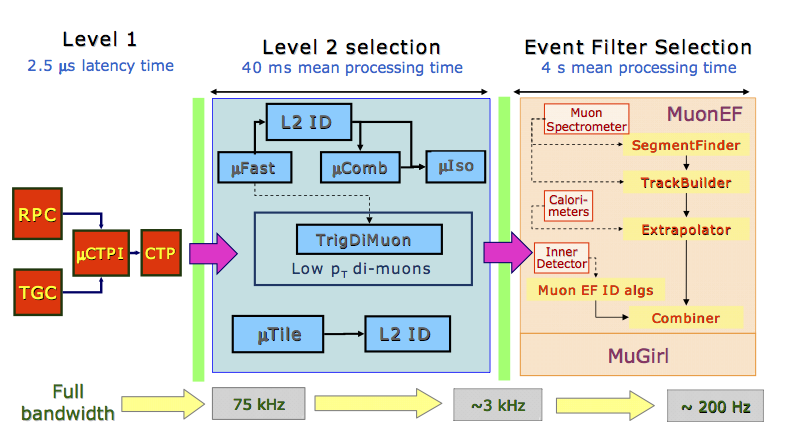
\includegraphics[width=\textwidth]{images/hlt_flow_muon.png}
    \caption[ Fluxo de dados entre os algoritmos do filtro de seleção para múons
    do ATLAS] {Fluxo de dados entre os algoritmos do filtro de seleção para
        múons do ATLAS (Retirado de~\cite{VENTURA2010}).}
    \label{fig:MUONHLTFLOW}
\end{figure}

\subsubsection{Algoritmos do L2 para Selecionar Múons}

O primeiro algoritmo do L2, o \emph{muFast}~\cite{DIMATTIA2003}, visa confirmar
ou descartar candidatos a múons escolhidos no L1. Através dele, são selecionados
tubos do MDT próximos a trajetória projetada pelo L1. Em cada estação, um ajuste
linear é realizado para obter a interseção entre a passagem do múon e a própria
estação, melhorando a reconstrução do trajeto percorrido pela
partícula~\cite{DIMATTIA2011}.

O algoritmo \emph{muComb} combina as informações provenientes do ID com a
trajetória do múon dentro do MS~\cite{VENTURA2010}. Desta maneira, é possível
extrapolar as trajetórias reconstruídas pelo ID até o MS e rejeitar múons
provenientes de decaimentos de píons e káons, assim como falsos alarmes e
raios-cósmicos~\cite{COSMICRAY2010}.


O terceiro algoritmo se baseia na informação extraída pelo \emph{muComb} para
refinar ainda mais a reconstrução do múon. Esse algoritmo, \emph{muIso}, é
utilizado para distinguir um múon isolado e um não isolado. Assim como o
\emph{muComb}, o \emph{muIso} pode ser utilizado para rejeitar múons oriundos de decaimentos
de hádrons. Porém, diferentemente do \emph{muComb}, informação de calorimetria é
utilizada~\cite{VENTURA2010}.


O \emph{muTile} foi implementado para aumentar a eficiência em múons com momento
transverso baixo. Para tal, ele baseia-se na energia depositada na última camada
do TileCal (célula D). Se a energia verificada for compatível com a de um múon,
então as demais células daquela torre são analisadas. Se o valor de todas as
células satisfazer os cortes energéticos do algoritmo, considera-se que a torre
foi cruzada por um múon~\cite{USAI2004}.

\subsubsection{Algoritmos do EF para Selecionar Múons}

Dois algoritmos fazem parte do filtro de eventos de múons: o \emph{TrigMuonEF} e
o \emph{TrigMuGirl}. Ambos são baseados nas ferramentas \emph{offline} de
reconstrução de múons~\cite{ARMSTRONG2004}.
Os algoritmos para deteção de múons do filtro de eventos seguem as mesmas
estratégias dos algoritmos do L2, contudo por possuir maior tempo de latência,
4~s contra 40~ms do L2, pode acessar mais informações e obter resultados mais
apurados. Assim, a principal tarefas deles é confirmar os candidatos de múons
validados pelo L2~\cite{VENTURA2010}.
